% !Mode:: "TeX:UTF-8"

\chapter{新的分层动态热管理方法的实现和结果比较}\label{sec:exp}

\section{新方法的实现}\label{sec:method_implement}
本论文中新的动态温度管理方法的实现是在一个具有两个 8 核 16 线程 CPU 的 linux 服务器上进行的,每个 CPU 主频为 2.90GHZ,服务器内存 64GB。
新的分层动态热管理方法主要用MATLAB实现。
我们分别构建了四个不同的处理器核配置的众核处理器,从 $100$ 核($10 \times 10$)到 $625$ 核($25 \times 25$)。
这些处理器的热模型由HotSpot生成,HotSpot已经有完整的工具可以直接调用。环境温度设定为 $20^{\circ}$C。
在这个实验中众核处理器由完全一致的Alpha 21264核组成。所有芯片的大小都是 $10mm \times 10mm \times 0.15mm$。
这里我们假设众核处理器中任务运行时相互之间没有通讯也不需要同步。
任务的功耗由Wattch通过运行SPEC基准程序  \cite{Henning:IEEEC'00} 生成,初始任务分配为,一个任务随机指定给一个核运行。
接下来的任务分配和调度有动态温度管理方法确定。
我们有9个SPEC基准程序的实时功耗信息。
对于不同的处理器的功耗信息,我们重复这9个功耗信息得到处理器需要的100个实时功耗信息,256个实时功耗信息等等。

因为核的大小会随核的数量增长变化,这会超过所谓的“功耗墙”或者“利用率墙”导致不现实的功耗密度  \cite{Taylor:MICRO'13} ,产生极高的温度。
为解决这个问题,提出了很多解决方法。一个解决方案是灰硅,放缩每个核的功耗  \cite{Huang:MICRO'11,Taylor:MICRO'13}。另一个更广泛的方法是完全关掉一些核\cite{Taylor:MICRO'13,Shafique:DAC'14}。
在我们的研究中,我们采用灰硅技术,放缩功耗的大小以保证所有处理器都有相似的功耗密度,这样温度分布就类似于现在的多核芯片。
这个可以通过以一定的比例调整操作频率和电压来实现,放缩比例在表~\ref{tab:param} 中给出。
在我们的这个研究中,我们并不考虑完全关掉一部分核的策略,这会是我们将来的研究方向。
\begin{table}[H]
\centering
\caption{对不同核数处理器在新分层方法的参数}\label{tab:param}{
 \begin{tabular}{|c|c|c|c|}
 \hline
 \hline
 处理器核数 &  放缩比例 & $e_{th}$ & $r$ \\
 \hline 
 \hline
 $100$ 核 ($10 \times 10$) & 0.21 & 0.06 & 500  \\
 \hline
 $256$ 核 ($16 \times 16$) & 0.08 & 0.05 & 2100 \\
 \hline
 $400$ 核 ($20 \times 20$) & 0.052 & 0.04 & 3000 \\
 \hline
 $625$ 核 ($25 \times 25$) & 0.033 & 0.03 & 3000 \\
 \hline
 \hline
 \end{tabular}
 }
 \end{table}
 
对于不同核数的处理器,为保证温度能有效地趋近顶温度,任务迁移过程中的阈值 $e_{th}$ 和 式 \eqref{eq:cost_fun} 中 MPC调整参数$r$ 需要手动调整。
这里注意,最优的 $e_{th}$ 和 $r$ 值与微处理器核的数量和结构高度相关,理论上没有必要去计算这些参数在实际的。
在实际的应用中,针对一个确定的众核微处理器,很容易通过实验来调整这些参数。
表~\ref{tab:param}给出了这些参数的值。我们可以看出 $e_{th}$ 随功耗模型的大小(在我们的情况中也是核的大小)变化。
如果核的大小相对较大, $e_{th}$ 也需要指定一个相对较大的值(即表~\ref{tab:param}中100核的情况)。反之亦然(即表~\ref{tab:param}中625核的情况)。
这是因为较大的功耗有较大的芯片空间供功耗分布,所以对相同的温度容忍限制,允许有更大的功耗差值。
另一个现象是核数越大,需要较大的 $r$ 值。
这是因为在式 \eqref{eq:cost_fun}中,当核数增长的时候$Y_{ceil}-Y_k$ 中的每个元素并没有变化太大,
但是 $\Delta P_k$ 中的每个元素会变得小很多(因为每个核的功耗缩小)。
为了使 $\Delta P_k$ 有更小的解, $r$ 的值需要变大。
这里注意625核的情况 $r$ 值仍然是 $3000$,与 $400$ 核的情况相同,因为我们发现到这个程度再继续增大 $r$ 值没有明显的影响。

在低层划分上,我们划分每 $25$ ($5 \times 5$) 个相邻核为一块。
在高层处理中,如果图 $\mathcal{G}_p$ 中的元素数目超过 $240$ 就用改进迭代最小割算法进行分割。

为了最小化任务迁移的开销,任务迁移和DVFS的启动周期设定为 $20$s。任务迁移的开销来自于计算核迁移操作。
通常处理器核数较小时,用较小的迁移周期。因为核数少时,计算开销和迁移操作开销(关系到核与核之间的通信)都很小。
对中核处理器情况,因为核数很大,频繁的任务迁移是很难执行的,所以迁移周期延长。迁移间隔内一个核的负载可能会增长很多,这样可能引起超出温度限制。
在这种情况下,我们在迁移间隔内需要保证安全的时候只能执行DVFS。

在实验中,除了任务迁移决策计算的开销,任务迁移操作的开销也要考虑进去。
正常的任务迁移操纵开销大概是 $10^6$ 个时钟周期,对 $1$GHZ的处理器大概是 $1$ms\cite{Cuesta:ISVLSI'10}。
因为在众核处理器中核数很大,核之间通信时间很长,这样的开销会很大。
所以我们设定上百核处理器的任务迁移时间为 $100$ms。
在实验中我们要考虑任务迁移的功耗。这个功耗由迁移时间内核的通信产生,在迁移时对应的两个核不处理任何任务。
所以我们假设任务迁移时间的功耗小于任务处理时间的功耗。为保证安全,我们将任务迁移时的功耗设定为之前处理任务时的平均功耗,用这样的功耗提供给MPC做预测。

作为比较,我们实现了另外两种基于MPC的方法,众核处理器基于MPC混合任务迁移和DVFS的动态温度管理方法 \cite{MaWang:APCCAS'14}和基于MPC只用DVFS的方法。
我们也选择了 \cite{Hanumaiah:TCAD'11}中的动态温度管理方法作为对比,因为它和我们的研究有相同的目标,即改性能处理器有温度限制时最大化性能(吞吐量)。
我们在实验中实现了开源项目 MAGMA V2,这个由 \cite{Hanumaiah:TCAD'11}的作者提供。MAGMA只能给出100核处理器的结果,对于更大的核数情况会有“超出内存”错误。
在这里所有的方法都用相同的激活周期,功耗信息和顶温度。

\section{与其他方法的瞬态温度比较}\label{sec:temp_comp}
首先我们不进行任何温度管理让100核处理器在最大速度上运行。图~\ref{fig:temp} (a)就是这个处理器的瞬态温度。我们可以看出,核的温度大概是从 $90^{\circ}$C
到 $120^{\circ}$C。温度在 $120^{\circ}$C 左右会影响芯片的可靠性。我们也测量了温度的方差,见图~\ref{fig:var_comp} (a)。可以看出,没有任何温度管理的情况下,核之间的温度差也很大。

\begin{figure}[H]
  \centering
    \subfigure[Temperature traces without any DTM method.]
  {
    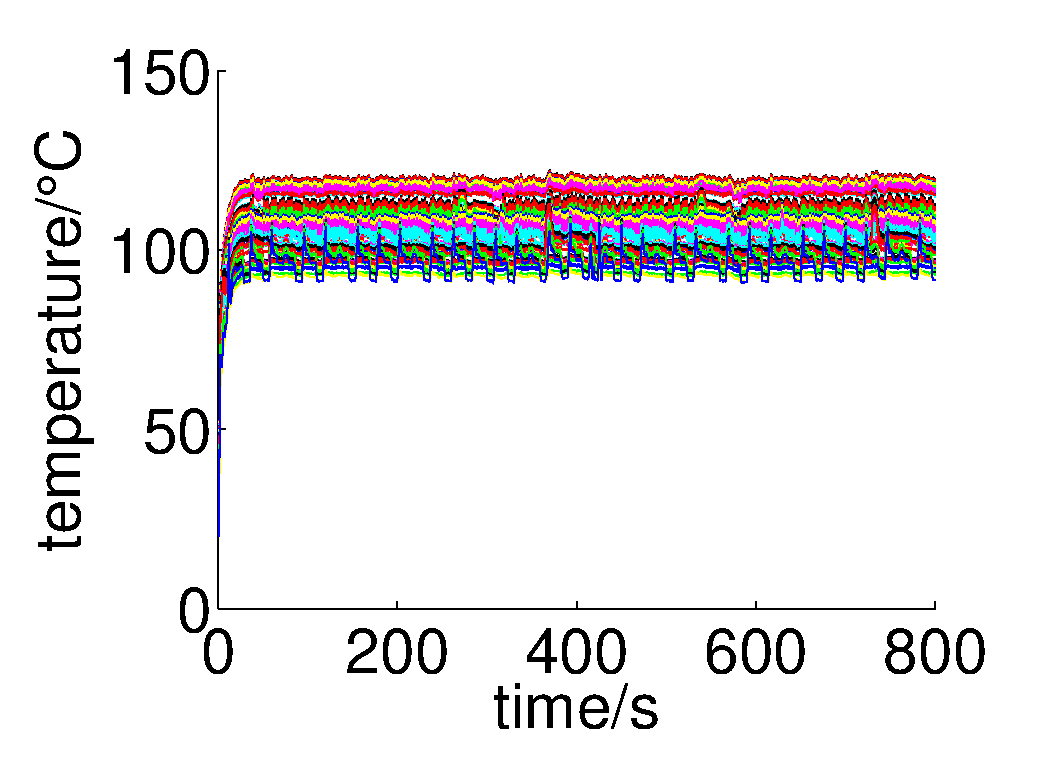
\includegraphics[width=0.32\columnwidth]{fig/T_bef}
  }
    \subfigure[Temperature traces with the new hierarchical DTM method activated at the $200$ second.]
  {
    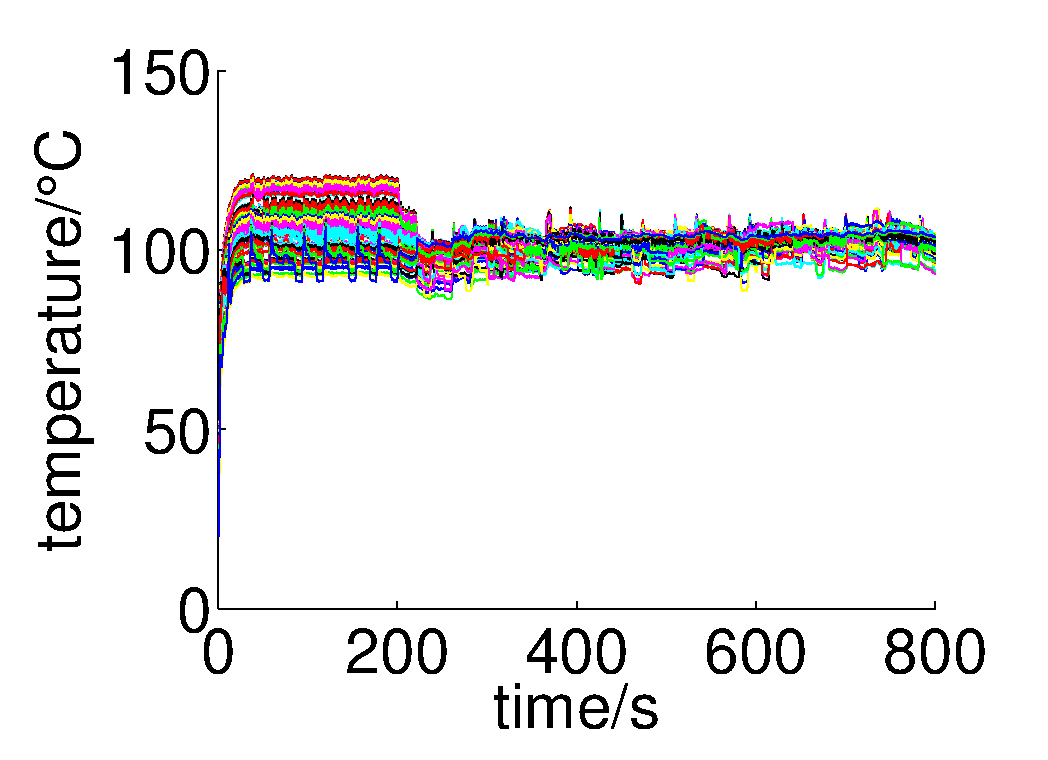
\includegraphics[width=0.32\columnwidth]{fig/T_aft}
  }
  \subfigure[Temperature traces with DTM method in cite \protect\cite{MaWang:APCCAS'14} activated at the $200$ second.]
  {
    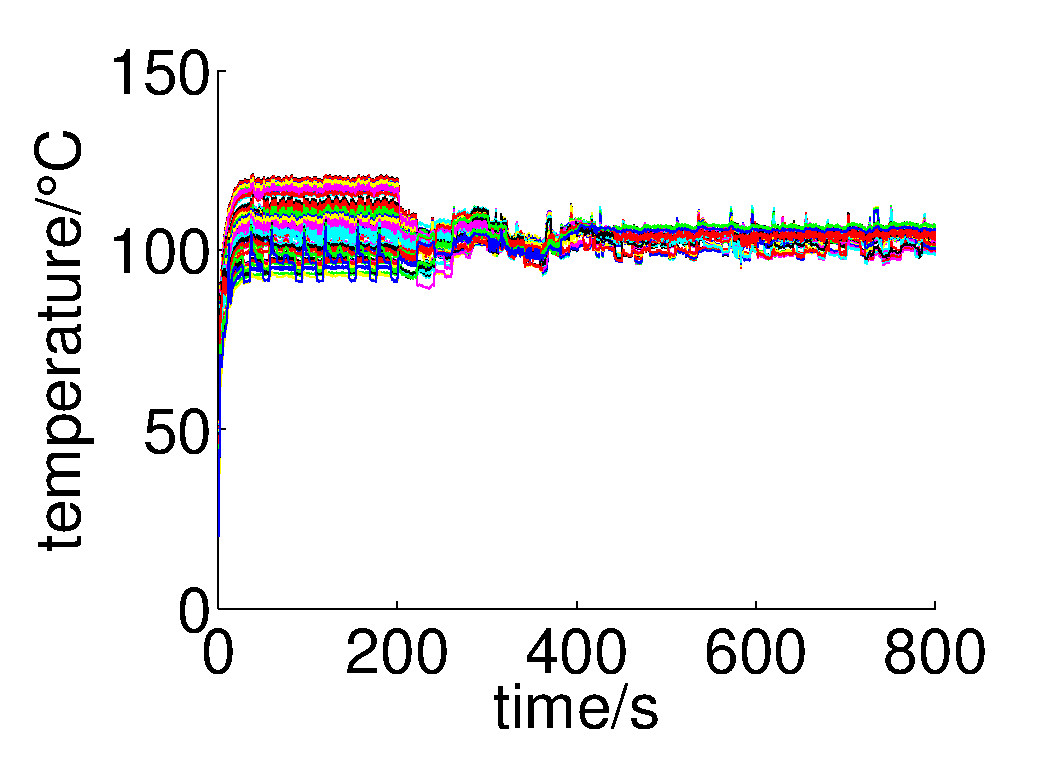
\includegraphics[width=0.32\columnwidth]{fig/T_cer}
  }
    \subfigure[Temperature traces with the DTM method with DVFS only activated at the $200$ second.]
  {
    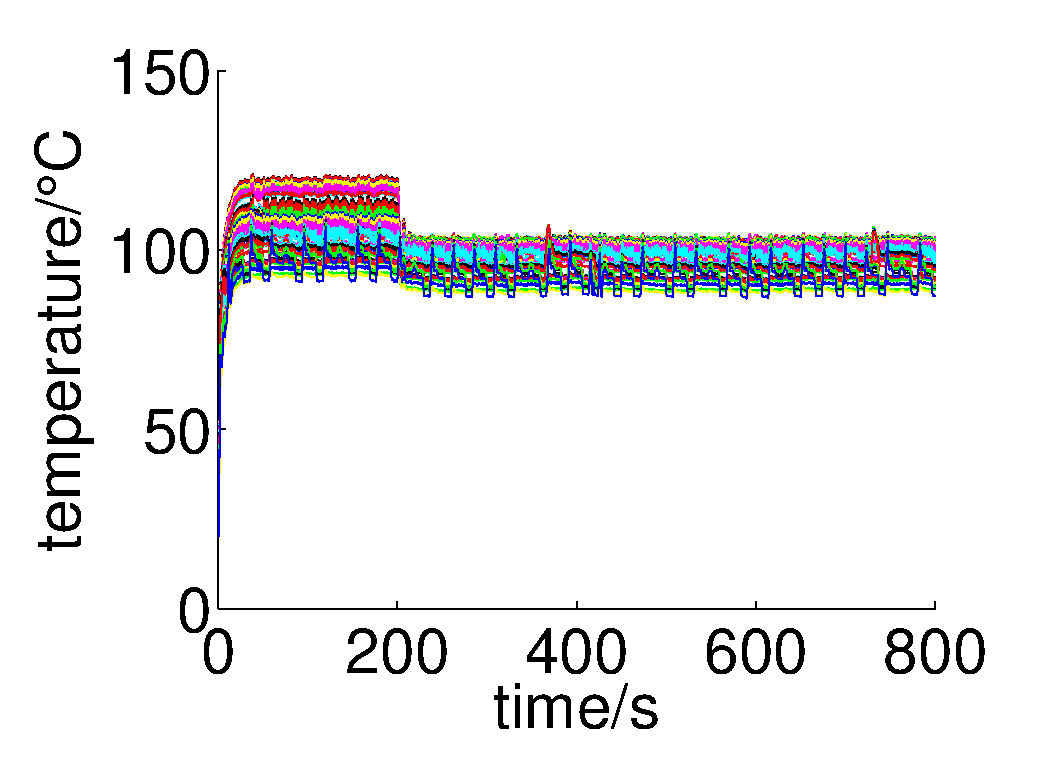
\includegraphics[width=0.32\columnwidth]{fig/T_dvfs}
  }

  \caption{Transient temperature traces of the $100$-core
    CPU with different DTM methods. Lines with different colors
    represents temperature traces of different cores. The new method
    in (b) and \cite{MaWang:APCCAS'14} in (C) both successfully tracks
    the ceiling temperature. But the DVFS only method in (d) has many
    low temperature cores, which means the chip performance is lower.}\label{fig:temp}
\end{figure}
\begin{figure}
  \centering
    \subfigure[The temperature variance without any DTM method.]
  {
    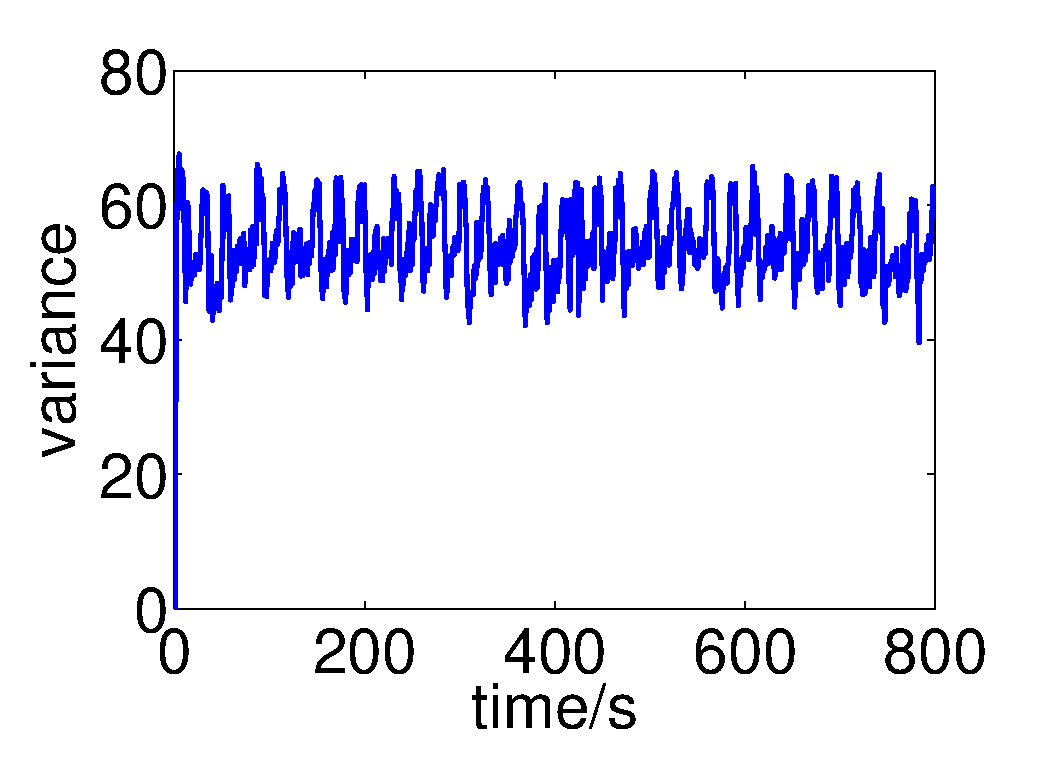
\includegraphics[width=0.32\columnwidth]{fig/var_bef}
  }
    \subfigure[The temperature variance with the new hierarchical DTM method activated at the $200$ second.]
  {
    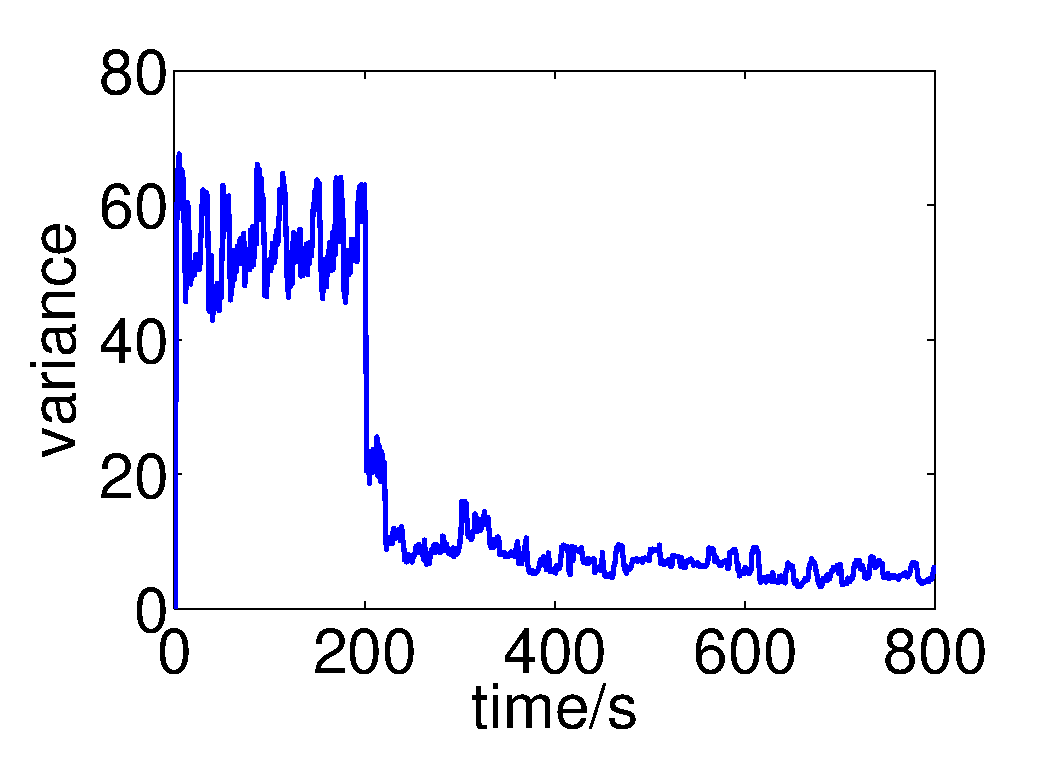
\includegraphics[width=0.32\columnwidth]{fig/var_aft}
  }
  \subfigure[The temperature variance with DTM method in \protect\cite{MaWang:APCCAS'14} activated at the $200$ second.]
  {
    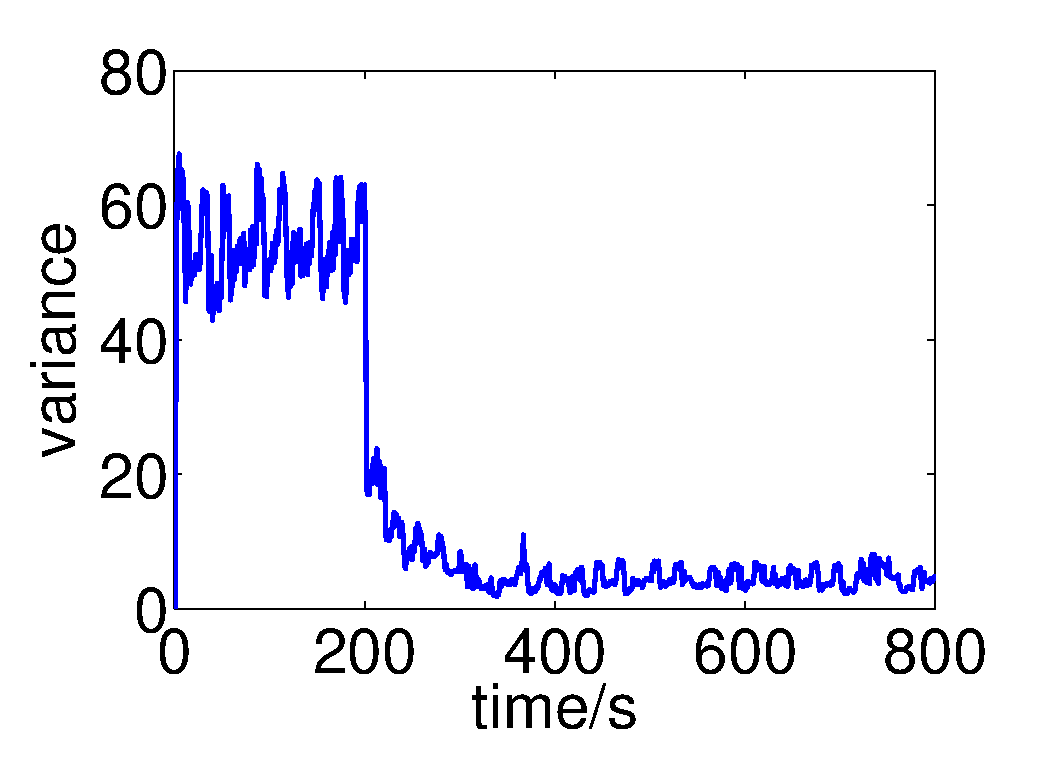
\includegraphics[width=0.32\columnwidth]{fig/var_cer}
  }
    \subfigure[The temperature variance with the DTM method with DVFS only activated at the $200$ second.]
  {
    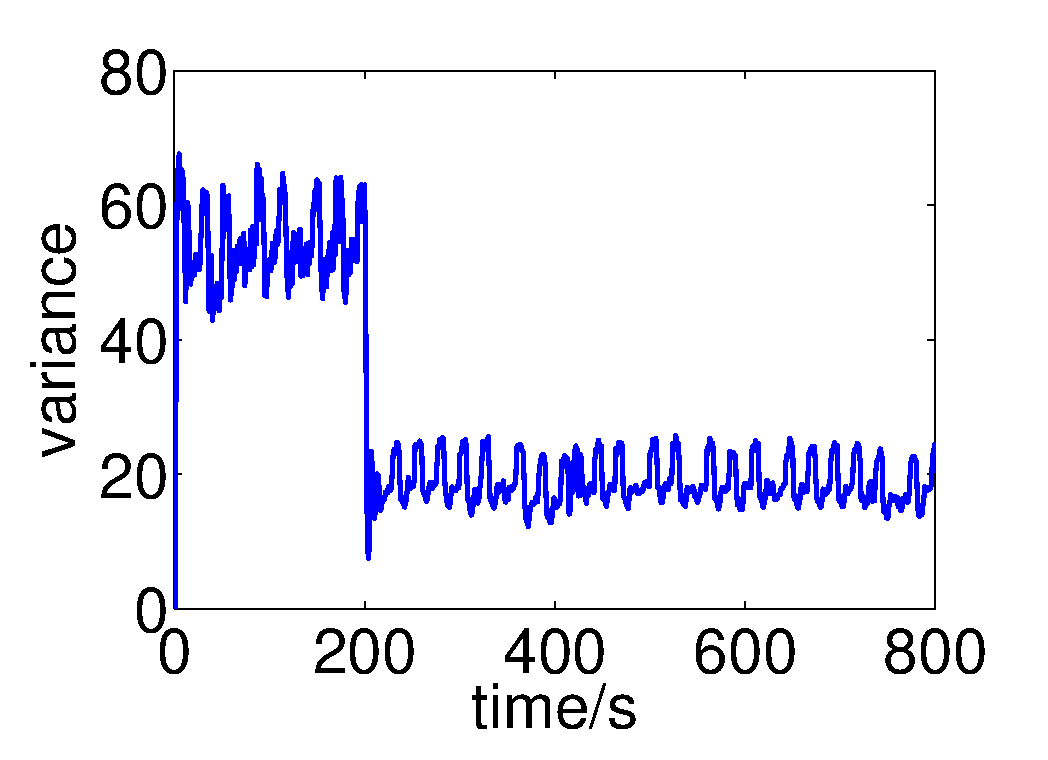
\includegraphics[width=0.32\columnwidth]{fig/var_dvfs}
  }

  \caption{Transient variances among cores in the $100$-core
    CPU with different DTM methods. The temperature variance of the
    new method is slightly higher than that of the method in
    \cite{MaWang:APCCAS'14}, but much lower than that of the DVFS only
  method.}\label{fig:var_comp}
\end{figure}

接下来我们把顶温度设定在 $105^{\circ}$C,测试新的分层动态温度管理方法在100核处理器上的效果。
分层动态温度管理方法在第200秒时被激活,激活周期为 $20$s。对应的瞬态温度就是图~\ref{fig:temp} (b),对应的温度方差就是图~\ref{fig:var_comp} (b)。
分层动态温度管理方法被激活之后,所有核的温度开始趋近于设定的顶温度 $105^{\circ}$C,核之间的温度差也减小了很多。

作为对比, \cite{MaWang:APCCAS'14}中的基于MPC的结合任务迁移和DVFS的动态温度管理方法和基于MPC结合DVFS的方法也进行了测试。
顶温度同样被设定为$105^{\circ}$C,所有的方法仍然在相同的时间点被激活,即第200秒,激活周期仍然是 $20$s。
图~\ref{fig:temp} (c) (d) 和 图~\ref{fig:var_comp} (c) (d)就是这两种方法对应的瞬态温度,和核之间温度方差。
我们提出的方法和 \cite{MaWang:APCCAS'14}中的方法有相似的瞬态温度,比 \cite{MaWang:APCCAS'14}中的核之间温度方差稍微大一点点(后面会介绍,新方法在开销和扩展性上比\cite{MaWang:APCCAS'14}要好得多)。
基于MPC结合DVFS的动态温度管理方法在瞬态温度和核之间温度差上要比前两种方法差很多。

下面我们对比 \cite{Hanumaiah:TCAD'11}中的方法。这个方法也是执行DVFS和任务迁移,来使核的温度趋近于顶温度。
不过,这个方法为了减小计算开销,在做动态温度管理决策的时候假设每个核都核其他核热隔离。这种假设在核数较少的多核芯片上或许可以,因为核数较少时,核之间有大面积的缓存区域阻隔了核间热交换。
但是在众核情况下,因为每个核面积较小,热交换很明显,并且不能被忽略。
该方法的100核处理器温度即图~\ref{fig:magma} (a)所示。因为这里的仿真步长较大,所以温度波形是直的线段。
依据这样的温度来做动态温度管理决策,温度大部分时间都是趋近顶温度的。
但是因为核与核之间的零热交换,所以这样的温度并不是实际的温度。
我们修改了MAGMA 程序,画出了考虑核间热交换的实际温度,如图~\ref{fig:magma} (b)所示。
我们很清楚地看到这个方法的动态温度管理决策不是优化的,会明显的超出实际温度的限制。
从图~\ref{fig:magma}我们可以看出,温度控制有一个延时调整问题。
这是因为在\cite{Hanumaiah:TCAD'11}的方法中,当当前温度并不完全等于顶温度的时候,核或者被关掉(如果当前温度高于顶温度),或者全速运行(如果当前温度低于顶温度)。
但是在图~\ref{fig:temp}中,所有基于MPC的动态温度管理方法都没有这个问题,因为它们可以提前预测来做决策,这样就会是比较平滑的温度控制。

\begin{figure}
  \centering
    \subfigure[Temperature traces of cores by assuming no heat exchange
    among cores.]
  {
    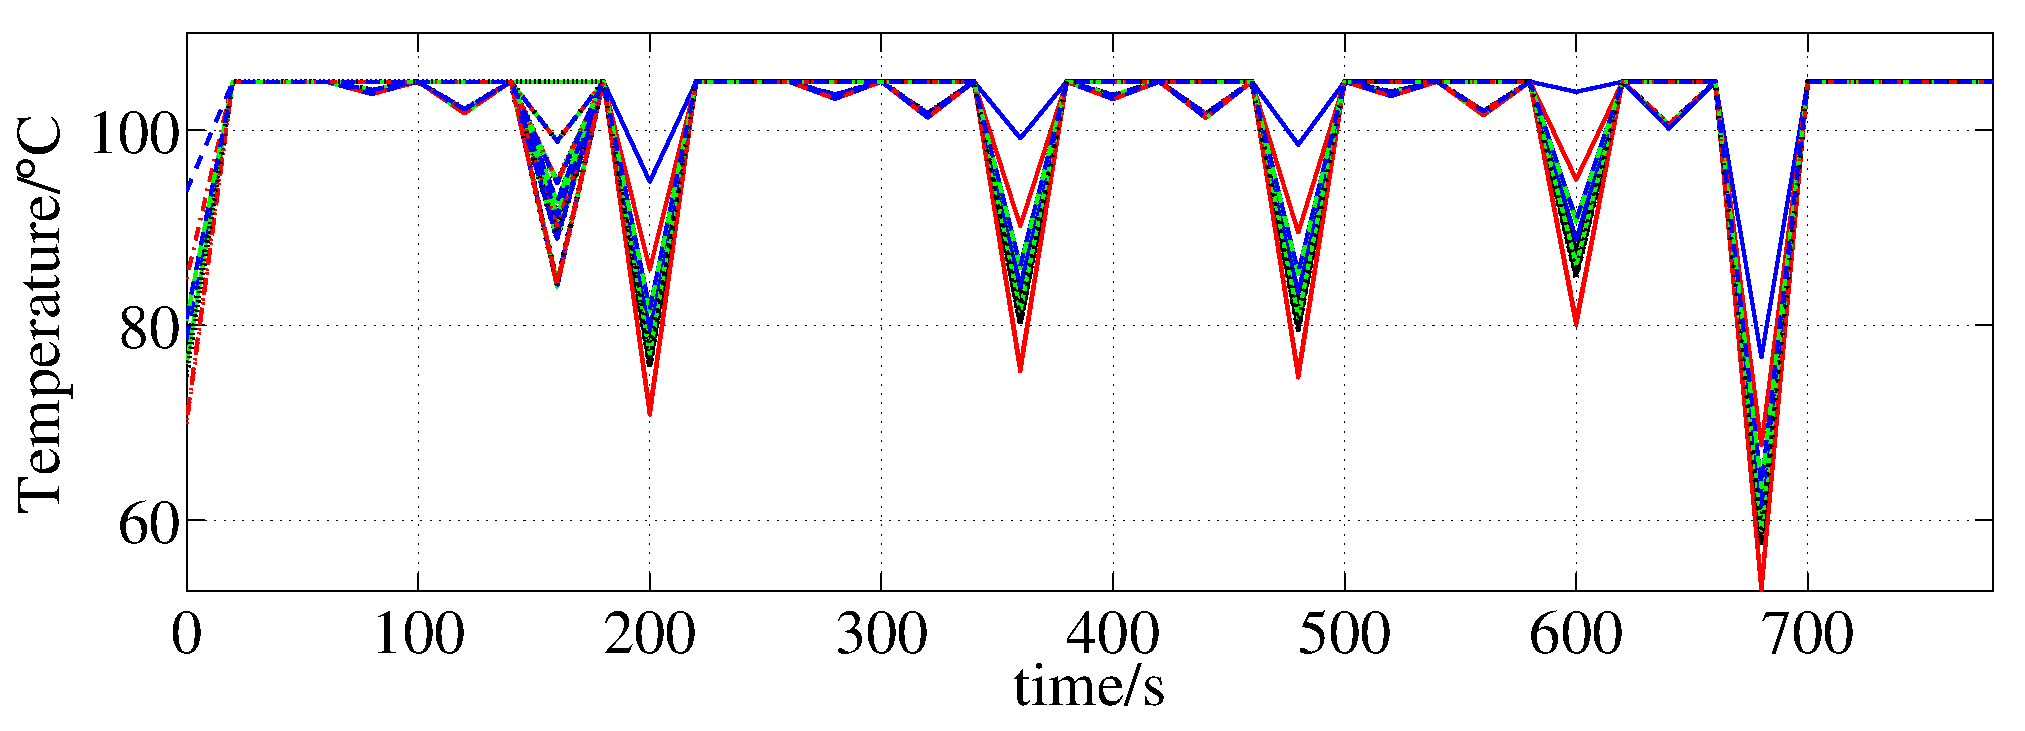
\includegraphics[width=0.7\columnwidth]{fig/magma_100_max}
  }
    \subfigure[Actual temperature traces of cores by enabling heat
    exchange among cores.]
  {
    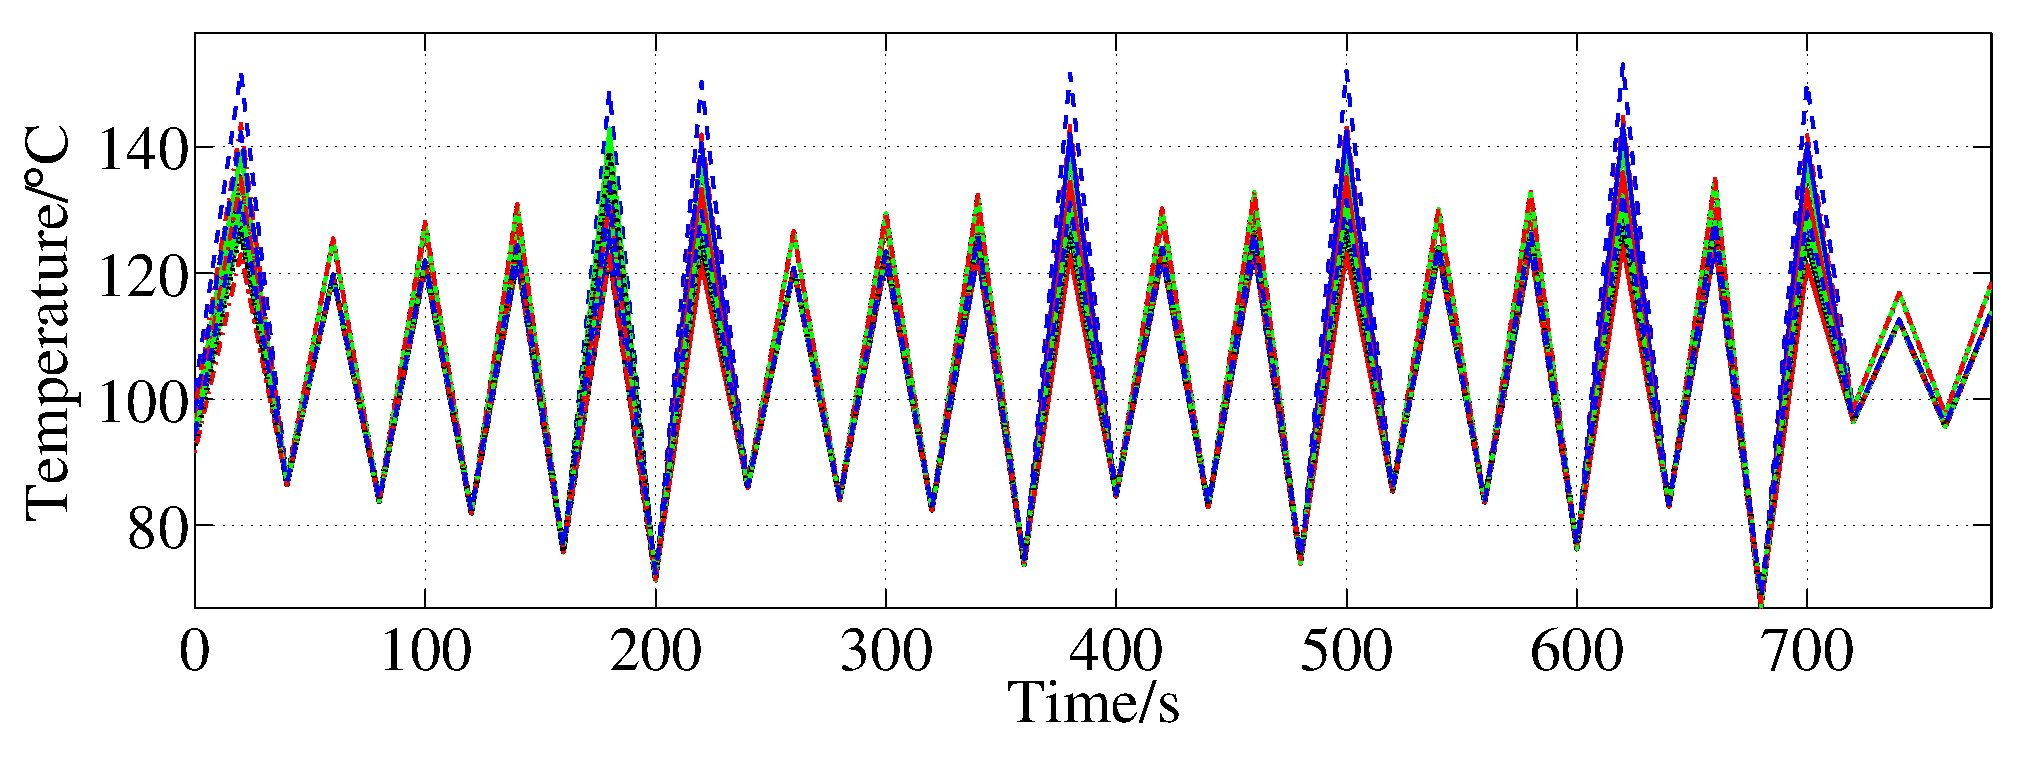
\includegraphics[width=0.7\columnwidth]{fig/comp_magma_100}
  }
  \caption{Transient temperature traces of cores by performing DTM in
    \cite{Hanumaiah:TCAD'11} on the $100$-core
    microprocessor. Core to core heat exchange has huge impact on
    temperatures for many-core microprocessors, causing the
    $105^{\circ}$C ceiling temperature to be seriously violated. Overshoot
    problem is also significant comparing to the MPC based techniques.}\label{fig:magma}
\end{figure}

表~\ref{tab:var} 记录了不同核数的处理器的核之间温度方差。表中 $var_o$ 是没用任何动态温度管理方法时核之间温度方差,
$var_d$ 是基于MPC只结合DVFS的动态温度管理方法的核之间温度方差,
$var_c$ 是 \cite{MaWang:APCCAS'14} 中动态温度管理方法的核之间温度方差,
$var_n$ 是我们的分层温度管理方法的核之间温度方差,
$var_h$ 是 \cite{Hanumaiah:TCAD'11} 中动态温度管理方法的核之间温度方差。
不同核数的结果类似, \cite{MaWang:APCCAS'14} 中方法稍微优于我们的分层动态温度管理方法,基于MPC只结合DVFS的方法明显有较大的核间温度方差。
\cite{Hanumaiah:TCAD'11} 中的方法只完成了 $100$ 核的实验,其核之间温度方差与 \cite{MaWang:APCCAS'14} 中的方法接近。

\begin{table}
\centering
 \caption{The temperature variance among cores in CPUs with different core
   configuration. $var_o$ is the variance without
any DTM method,  
$var_d$ is variance with DTM using DVFS only, 
$var_c$ is variance with DTM in \cite{MaWang:APCCAS'14}, 
and $var_n$ is variance with our
new hierarchical method, and $var_h$ is the variance with method in \cite{Hanumaiah:TCAD'11}. \label{tab:var}}{
 \begin{tabular}{|c|c|c|c|c|c|}
 \hline
 \hline
 %%Distribution  & $var_o$ & $var_d$ &$var_n$ & $P_d$ & $P_n$ \\
 Configuration  & $var_o$ & $var_d$ & $var_c$ & $var_n$ & $var_h$ \\
 \hline 
 \hline
 $100$ 核 ($10 \times 10$) & 54.2 & 18.8 & 5.5 & 7.6 & 5.9\\

 \hline
 $256$ 核 ($16 \times 16$) & 50.8 & 19.3 & 3.4 & 6.5 & N/A\\
 \hline
 $400$ 核 ($20 \times 20$) & 52.1 & 16.7 & 2.5 & 4.1 & N/A\\
 \hline
 $625$ 核 ($25 \times 25$) & 50.5 & 15.9 & 2.3 & 4.1 & N/A\\
 \hline
 \hline
 \end{tabular}}
 \end{table}
 
 \section{与其他方法的算法执行时间比较}\label{sec:time_comp}
 
 从前面的比较可以看出,我们新提出的分层动态温度管理方法与 \cite{MaWang:APCCAS'14}中的方法在瞬态温度和核之间温度方差上的相差不大。
 在众核处理器上与 \cite{MaWang:APCCAS'14}、 \cite{Hanumaiah:TCAD'11}相比,我们的新方法真正的亮点是可扩展性和小开销。
 我们测定这几种算法的平均每秒执行时间。
 我们的新方法主要由MPC,二部图匹配(任务迁移),最小割划分组成。为更好分析,我们将算法的总执行时间分为MPC时间 $t_p$ ,匹配时间 $t_m$ ,最小割划分时间 $t_a$ 。
 匹配操作的执行时间一部分为低层匹配时间,另一部分为高层匹配时间。对于低层匹配时间,如果这里有多个匹配操作在并行执行,我们只计最长的一个,这个时间才是主导延时的时间。
 \cite{MaWang:APCCAS'14} 中的方法也有MPC时间 $t_p$ 和匹配时间 $t_m$ ,但是没有最小割划分时间 $t_a$ 。
 只用DVFS的方法只有MPC时间 $t_p$。
 尽管 \cite{Hanumaiah:TCAD'11} 中的方法只完成了100核的情况,但是我们还是可以测试它的任务迁移时间 $t_m$ 。我们可以用正确维度的随机矩阵输入给对应的函数。
 表~\ref{tab:time}记录了各算法在不同核数处理器上的执行时间。很显然随核数增长, \cite{MaWang:APCCAS'14} 中的方法开销明显上升。
 从400核的情况开始,每秒的平均管理决策时间要超过1s,这是完全不能接受的。
 \cite{Hanumaiah:TCAD'11} 中的方法在任务迁移计算上的时间也随核数很快增长,使它不能扩展到众核应用中。
 根据这篇论文,我们找出任务迁移算法的时间复杂度为 $O(nq)^3$(跟 \cite{MaWang:APCCAS'14} 中的任务迁移算法接近),其中$n$是核数,$q$是任务数量。
 这篇论文中假设 $n=q$ ,那么当核数增长额时候, $O(n^6)$ 的复杂度使任务迁移占用了太多的时间。
 相对地,我们新的分层算法的计算时间增长缓慢。即使是625核的情况(这已经是很大的核数了),我们的方法平均每秒消耗 4 ms 做管理决策。
 这仅仅是 $0.4\%$ 的计算时间花费在少数几个核上,因此这个可以被忽略。
 当然,仅仅用DVFS的方法需要最少的时间计算开销,但是我们的新方法只在任务迁移上花费很少的开销就使性能显著提成,下面将继续介绍。
 
  \begin{table*}[h]
\tabcolsep=2pt
 \caption{The average runtime per second of the DTM methods on CPUs with
   different core configurations. $t_p$ represents MPC time, 
$t_m$ means task migration matching time, and $t_a$  denotes for minimum cut partitioning time.\label{tab:time}}{
 \begin{tabular}{|c|c|c|c|c|c|c|c|c|c|c|c|}
 \hline
	        & \multicolumn{4}{c|}{分层方法} & \multicolumn{3}{c|}{\cite{MaWang:APCCAS'14}} & \multicolumn{2}{c|}{仅DVFS方法}& \multicolumn{2}{c|}{\cite{Hanumaiah:TCAD'11}} \\
 \hline
核数	& $t_p$ & $t_m$ &$t_a$ &
$t_{all}$ & $t_p$ & $t_m$ &$t_{all}$  &
$t_p$ &$t_{all}$ & $t_{m}$ &$t_{all}$\\
                               &   $(10^{-4}s)$ & $(10^{-4}s)$ &
                               $(10^{-4}s)$ & $(10^{-4}s)$ & $(10^{-4}s)$
                               &   $(s)$  & $(s)$  & $(10^{-4}s)$ & $(10^{-4}s)$ &   $(s)$  & $(s)$\\
 \hline 
 \hline
$100$ & 1.58 & 1.63  & 0     & 3.21 & 1.49 & 0.01 & 0.01 & 1.60 & 1.60 & 0.01 & 0.01\\
 \hline
$256$ & 2.85 & 19.26 & 1.58  & 23.7 & 2.93 & 0.45 & 0.45 & 2.80 & 2.80 & 0.09 & 0.09\\
 \hline
$400$ & 4.88 & 7.77  & 3.27  & 15.9 & 5.38 & 1.90 & 1.90 & 5.29 & 5.29 & 0.34 & 0.34\\
 \hline
$625$ & 9.09 & 12.27 & 17.49 & 38.8 & 8.27 & 8.63 & 8.63 & 8.87 & 8.87 & 0.99 & 0.99\\
 \hline
 \hline
 \end{tabular}}
 \end{table*}

\begin{table}[h]
\centering
 \caption{The average number of instructions per second of one core on
   CPUs with different configurations. $MIPS_o$ represents the IPS in million (MIPS) of the core without any DTM method,
$MIPS_d$ is for MIPS of DTM with DVFS only,
and $MIPS_n$ denotes MIPS of our new hierarchical method.\label{tab:ips}}{
 \begin{tabular}{|c|c|c|c|}
 \hline
 \hline
 Configuration  &$MIPS_o$ & $MIPS_d$  & $MIPS_n$ \\%&  \textcolor{red}{$MIPS_h$} \\
 \hline 
 \hline
 $100$ cores ($10 \times 10$) & 290.8 & 279.6 & 281.5 \\%& \textcolor{red}{231.9}\\
 \hline
 $256$ cores ($16 \times 16$) & 210.2 & 202.9 & 207.1 \\%& \\
 \hline
 $400$ cores ($20 \times 20$) & 182.1 & 174.7 & 178.8 \\%& \\
 \hline
 $625$ cores ($25 \times 25$) & 156.5 & 150.2 & 154.4 \\%& \\
 \hline
 \hline
 \end{tabular}}
 \end{table}
 
 \section{与其他方法的性能比较}\label{sec:ips_comp}
 
 最后我们测定不同众核处理器采用各种动态温度管理方法的性能。
 每秒执行的指令数(IPS)是衡量处理器性能一个标准。
 因为 \cite{MaWang:APCCAS'14} 和 \cite{Hanumaiah:TCAD'11} 中的方法有很大的开销,不能完成众核处理器的管理决策,
 所以在性能对比中并没有考虑这两个方法。
 表~\ref{tab:ips} 记录了采用新分层方法和仅采用DVFS的方法时的平均 IPS。
 在表中 , $MIPS_o$ 表示不采用任何动态温度管理方法时单个处理器核的平均IPS(以百万计就是MIPS),
 $MIPS_d$ 表示采用DVFS方法时单个处理器核的平均IPS,
 $MIPS_n$ 表示采用我们的新方法时单个处理器核的平均IPS
 $MIPS_o$ 是理想性能,是在处理器没有任何温度限制的情况下取得的。
  $MIPS_n$ 只比  $MIPS_o$ 小一点,说明在确定管理决策时,我们新的分层算法是很有效的。
  从表中可以看出,我们的新算法在性能上优于只采用DVFS的算法。
  尽管新算法有稍微大一点的开销,但是消耗在任务迁移决策的时间减少了DVFS激活的次数,带来的是性能收益。
  我们注意到,新方法相比于DVFS方法在吞吐量上的提升和运行的应用有很大关系。
  比如,如果这里有很低温度的核(甚至是闲置无任务的核),新方法就会比DVFS方法有更明显的吞吐量提升,
  因为低温核可以被任务迁移充分利用,减少DVFS操作。
  
 
 
 
 
 
 


























